\chapter{Adaptive Learning}
\label{chap:adaptive-learning}

% TODO:
% - incorporate other notes from my/thesis gdoc
% - inspiration from relevant articles
% - add references for provided examples (playing chess, autonomous car, ...)

From playing chess to driving an autonomous car,
  artificial intelligence proved to be a mighty tool
  for tackling difficult algorithmic tasks.
The power of artificial intelligence can be also used
  to develop a personalized adaptive system for learning programming.
Such system would create an optimal learning experience for each student
  by providing them with problems of difficulty matching their skill,
  so that the student stays challenged and interested in solving them.

TODO: terminology note: Intelligent tutoring systems (ITS)
  (REF e.g. Hyacinth S. Nwana. Intelligent tutoring systems: an overview)
  (? is ITS = adaptive learning system, or is AL too specific term - just
  one of more possible strategies?)

In the existing systems (\ref{sec:existing-systems}),
  the sequence of tasks is the same for everybody.
As a result, the progress is necessarily too slow for some students,
  who could skip some of the tasks,
  while being too fast for others,
  who could highly benefit from solving a couple of other similar tasks.
Artificial intelligence can be used to personalize
  the sequence of tasks for every student.
By giving the student a suitable task
  -- neither too easy, nor too difficult --
  it can help the student to get into the state of flow
  (\ref{sec:motivation.challenge}).

In addition to choosing the most suitable task for given student,
  artificial intelligence has also other possible uses in learning systems,
  for example automatic hints generation \cite{generating-hints},
  cheating detection (REF),
  or skills visualization (REF).
Furthermore, artificial intelligence techniques can be used
  to analyze collected data offline.
Such analyses can reveal problematic tasks,
  or suggest how to group tasks into problem sets (TBA: ref).

Adaptive learning systems have been already successful in some domains.
For instance, Map Outlines%
  \footnote{Available at \url{https://outlinemaps.org}.},
  developed by Adaptive Learning research group at Masaryk University,
  is an intelligent web application for learning geography.
It has been used by tens of thousands of students
  and online experiments have confirmed
  that the adaptivity of the system helps to improve the learning outcome
  \cite{alg.evaluation-geography}.
In addition to geography, similar adaptive web applications
  for learning anatomy%
  \footnote{Available at \url{https://practiceanatomy.com}.},
  biology%
  \footnote{Available at \url{https://poznavackaprirody.cz} (in Czech only).},
  elementary mathematics%
  \footnote{Available at \url{https://matmat.cz} (in Czech only).},
  and Czech grammar%
  \footnote{Available at \url{https://umimecesky.cz} (in Czech only).},
  were developed by the research group in recent years.

TODO:
- mention other famous ITS (Duolingo);
- specifically name ITS' related to programming - refs to the previous
chapter (Umime programovat, Tutor)


Sections \ref{sec:domain-modeling} and \ref{sec:student-modeling} present how
to model the domain and students of the introductory programming.
Sections \ref{sec:task-recommendation} and \ref{sec:mastery-learning}
then describe two different uses of these models to make a learning system
personalized, namely adaptive task recommendation, and mastery learning.
Finally, section \ref{sec:metrics-and-evaluation} discusses how to evaluate
different models or even whole learning systems.

\subsection{Terminology}

TODO: move to a most suitable place

\begin{itemize}
\item \emph{Student} (learner) -- TODO.
\item \emph{Task} (item, problem)
  -- a problem presented to the student to solve.
  Consists of setting, sample solution (and has a \emph{difficulty}).
  (REF figure with an example from previous chapter)
\item \emph{concept} (knowledge component, chunk)
  -- knowlege (ability) such as loops or conditionals,
  (together with tasks for practicing this ability?,
   maybe: chunk = concept togehter with tasks to learn that concept)
\item \emph{Task Set} (problem set)
  -- a group of tasks for practicing a concept (chunk?).
  (TODO: remove this term if not used)
\item \emph{Skill}
  -- how well a chunk is mastered by a student.
\item \emph{Task Session}
  -- a noninterrupted attempt of a student to solve a task.
  (attributes: success, time, program snapshots)
\end{itemize}

TODO: figure illustating all these terms

TODO: type of chunks: tasks, problem sets (missions, phases), programming concepts,
  syntax concpets (blocks), game concepts, (misconceptions), mastery,
  (NOTE: KLI framework also describes the differences between these different types
  of chunks, which they call knowledge components; + also granularity levels)

KLI framework (Koedinger 2012), KCs with examples for programming:
- variable-variable (principle):
  - very coarse: programming
  - coarse: loops
  - medium: while loops
  - fine: programs with single while-not-end loop
- variable-constant (category):
  - coarse: game elements and mechanics?
  - medium: asteroid?, winning rule?
  - fine: ?
- constant-constant (fact):
  (names of game elements / names of parts of the environemnt / names of programming blocks),
  (behavior of game elements, e.g. what happend when you hit the asteroid)

\subsection{Components}

TODO: high-level description of components + REF sections below
REF: source of the division, e.g. \cite{its-learner-models}

\begin{itemize}
\item \emph{Domain model} -- concepts, tasks and relationships between them
    (possibly also misconceptions, rules for solving the tasks).
\item \emph{Student model} (learner model, user model) -- performance on tasks, skills of concepts.
\item \emph{Tutor model} (instructional policy, instructional strategy, pedagogical module) --
  decides what given student in given domain should do next (e.g. task recommendation).
\item \emph{User interface model} (tutor-student interface) -- how the domain, student and tutor models should be presented to the student (e.g. task solving environment, overview of all tasks and concepts, achieved skills, recommended task).
\item \emph{Sensor model} - collecting data from the interactions with the system
  (includes monitorin?).
\end{itemize}

I think there are two more components of ITS:
\begin{itemize}
\item \emph{Online analysis/experiment/evaluation/hyperparams training layer/module} -- AB experiments, online hyperparams tuning.
\item \emph{Offline analysis/evaluation/training} (Human in the loop - but part
  of the online analysis includes human-in-the-loop as well).
\end{itemize}

TODO: diagram of the components (+ used data):
- domain model <- all historical data;
- student model <- student historical data, domain model
- tutoring model <- domain model, student model
- experiment layer (online analysis) <- all 3 models (possibly collections if it compares multiple ones) (possibly also UI model)
- UI <- results from all models (but usually not the actual models) (structure from the domain model for overivew of tasks, skills and mastery from the student model, recommendation from the tutoring model), these models can be selected by the experiment layer
- ? forward pass (system->student) vs. backpropagation through the models (student->system -> online parameters update)
- ? models vs. real entities (student model vs. student, UI model vs. UI)


NOTE: online vs offline models: for domain and tutoring, offline models are ok, for student, online models are necessity


\imgW{its-components}{Components of ITS with their input and output}


\section{Domain Modeling}
\label{sec:domain-modeling}

\begin{itemize}
\item Domain model is a collection of educational content, covered concepts,
  relationships between them, and an algorithm to learn
  parameters of the model from data.
  (TODO: improve the definition, REF to examples)
\item Usage:
\begin{enumerate}
\item In student models: provides structure for student skills and describes relationships between them, which can be used to predict a performance of student with given skills on given task.
(This is useful for example for skill transfer -- after observing performances on a few tasks,
    performance on other tasks can be inferred using the relations between the solved and
    unsolved tasks described by the domain model.)
\item In tutor models, e.g in mastery learning, we can select a task from a practiced concept until the concept is mastered (so we need to know which tasks contain each concept).
\item In user interface, e.g. grouping tasks into problem sets,
  or providing a rich open learner visualization (in conjungtation with the student model).
\item In online/offline analysis (human-in-the-loop) for actionable insight
    (e.g. we can find that a task behaves very differently than all others in
    the same problem set, so we will explore the task and find a bug in its setting,
    such as a missing limit, which makes the task much easier then expected).
\end{enumerate}
\item Appropriate model depends on the usage (no single best domain model),
  so it may be useful to have multiple domain models inside a single system
  (but the cost of creating and maintaining multiple domain models is a consideration).
\item Comprehensive overview of domain modeling approaches e.g. in \cite{its-domain-models}
  (here we focus specifically on the domain of introductory programming).
\end{itemize}


\subsection{Domain Data}
% consider: "Chunks", "Chunks and Relationships", "General Chunk Model", "Domain Ontology"

\begin{itemize}
\item Input data (vs. model data) -- content + collected (historical) data.
\item Content:
  task statement (including name and world description),
  sample solution, labels (e.g. covered concepts), problem sets.
\item Historical: observations (REF to discussion on performance in student models section).
\item Model data: chunks and relationships between them.
\item Chunks = all entities in the domain:
\begin{itemize}
\item tasks,
\item other educational content (text, videos, interactive visualizations),
\item problem sets (group of tasks usually presented in the user interface),
\item concepts (aka. knowledge components, learning objectives; e.g. loops),
\item misconceptions (e.g. "if-statement is a loop").
\end{itemize}
\item In addition to content attributes (e.g. setting, description),
    parameters can be associated with chunks, for example:
\begin{itemize}
\item median time,
\item difficulty (?),
\item mastery threshold.
\end{itemize}
\item Furthermore, relationships between chunks can be me modeled:
\begin{itemize}
\item inclusion/part-of (e.g. problem set contains tasks, tasks contain
  concepts (Q: direction?))
\item generalization/subclass (e.g. programming is a more general concept than loops),
\item prerequisiites (e.g. single loops are prerequisity for nested loops).
\item TODO: Q: what is the interpretation of the edges in BN
  (vaguely it's something like "influence", or "directly depend on";
   missing edges encodes conditional independence (given the parents))
\end{itemize}
\item The graph of entities with the binary relationship betweeen them is
  called \emph{semantic net} (in the field of knowledge representation).
\item Useful concept in semantic nets is \emph{inheritance}:
  properties of classes also holds for their subclasses and instances (transitively),
  unless an exception is specified.
  For example, instead of setting the same set of allowed blocks in each task
    in a problem set, it is enough to specify that toolbox only in the problem set.
    However, if there is a task in the problem set that needs to add one special block,
    it can override the default toolbox.
\item All of these relationships can be either hard (binary) or soft (continuous).
\item Modeling decisions: which type of chunks, (which parameters of chunks),
  which relationships, how to set/compute the values (e.g. structure between
  chunks, values of similarities between tasks), (interpretation/semantics?).
\end{itemize}

TODO: nonbinary relationships? needed for example to express CPTs in unconstrained BN

TODO: ontologies (= formal description of terms and relationships betwwen them
in given domain; -> knowledge graphs; knowledge representation field), Bayes Nets

TODO: note: historical data vs. domain data (domain data = "compressed" version of
  "input data" (provided by content creators) and historical data.

\subsection{Algorithms}

\begin{itemize}
\item all but the simplest domain models contain some parameters,
  which can be either set manually or learned from collected data
\item domain model = data (chunks, parameters, relationships) + algorithms:
  (REF: overview of components in \cite{pelanek-learner-modeling})
\item 3 types of algorithms:
\begin{enumerate}
\item \emph{learning} domain data based on historical data
\item \emph{inference} based on the domain data
  (? basically semantics/interpretation of the data)
  (e.g algorithms for mapping prerequisites to acceptance decision;
    for mapping task performances to a concept skill/mastery,
    for aggregating skills to a parent concept skill in a hierarchical model)
\item ? getting \emph{insight} through visualization techniques
    (e.g. projections to plane, TODO: add t-sne example)
\end{enumerate}
\item inference must be fast (in our case the domain is small, having tens or
  hundreds of chunks, then linear complexity wrt. to the domain size is ok),
    learning and insight algorihtms can be slower
    (e.g. linear wrt. to the size of historical data)
\end{itemize}

Learning:
\begin{itemize}
\item what we can learn: parameters (usual), structure = relationships and
  chunks (less usual, because it requires more data)
\item learning algorithm can be offline
  (once enough data is collected, parameters are quite stable)
\item need to deal with new tasks (set their parameters by an expert or a content-based heuristic)
\item extension: online update of the parameters (useful if a lot of new tasks
  are introduced often, which is not our case)
\end{itemize}


\subsection{Tasks}

\begin{itemize}
\item aka problems, items
\item name, setting, and solution
\item parameters (features) --
  computed from setting (e.g. size of the grid),
  solution (e.g. length of the solution),
  and performance data (e.g. median time).
\item TODO: tasks pool visualization (projection) -- add plot
\end{itemize}

\subsubsection{\textbf{Concept-free Models}}
\begin{itemize}
\item = all task are assumed to cover a single indivisible concept (e.g. "programming")
\item the simplest domain model = only tasks (no other chunk types) and no relationships
\item oven without concepts, the models can have
  rich structure (e.g. prerequisities between tasks,
    see right figure \ref{fig:chunks-prerequisites})
  and many parameters (e.g. similarities between tasks)
\item REF: usage (most of the existing systems)
\end{itemize}


\subsection{Concepts}

\begin{itemize}
\item (motivation) The assumption of a single concept for all tasks is
  reasonable for many logic puzzles (e.g. sudoku), but not in programming.
  For example, it is possible to master loops while struggling with functions,
  and vice versa.
\item TODO: define/REF
\item aka knowledge components \cite{knowledge-components}
\item granularity: while-loop < loops < programming
\item modeling decisions: which concepts, how granular, what are the
  relationships between them, which tasks belong to which concepts?
\end{itemize}

\subsubsection{\textbf{Disjoint Concepts}}
\begin{itemize}
\item task:concepts 1:m (each task in execatly 1 concept)
\item aka "concept model", "flat concepts" (concepts are flat clusters of tasks)
\item Concepts can be either defined manually or detected automatically
  (REF: \cite{niznan-thesis, rihak-phd}, spec.pages),
\item automatically: a clustering algoritm (e.g. k-means, k-medoids, spectral clustering)
  operating on task-features or task-task similarity matrix
  (REF: our paper about similarity of programming problems)
\item or semiautomatically, improving upon a mapping from tasks to concepts
    provided by an expert \cite{its-domain-models}, chapter 3).
\item Manually selected concepts, such as loops and conditional commands,
  have the advantage of being interpretable,
  so they can be used for skills visualizations in the user interface
  to provide students with the information about their learning progress.
  Furthermore, no data needs to be collected in advance,
  while the automatic techniques require a lot of data to provide stable results.
  (TODO: specify "a lot of" + REF).
\item example in figure \ref{fig:concepts-disjoint-overlapping} (left)
\item REF: usage (? ProSo - single concept per problem type, e.g. all tasks in Robotanist are single concept)
\end{itemize}

\imgW{concepts-disjoint-overlapping}{Comparison of disjoint and overlapping concepts.}

\begin{figure}[htb]
\begin{center}
  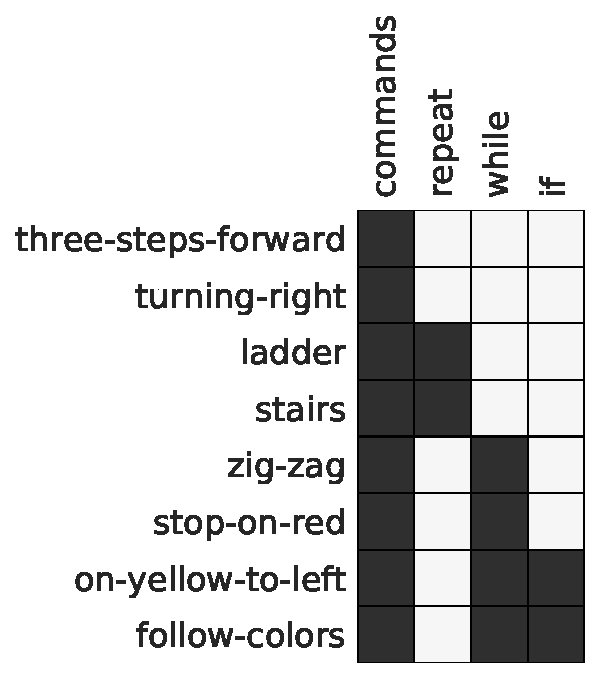
\includegraphics[width=0.42\textwidth]{img/qmatrix-binary}
  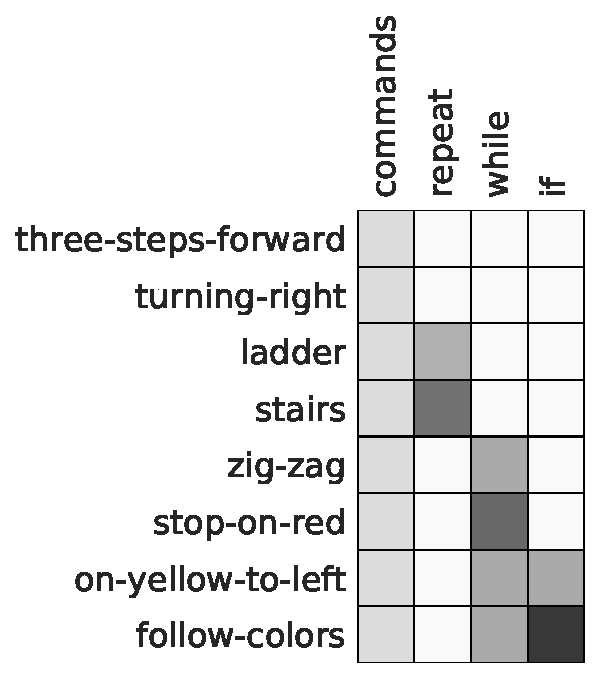
\includegraphics[width=0.42\textwidth]{img/qmatrix-continuous}
\end{center}
\caption{%
  Binary and continuous Q-matrix corresponding to the
  bipartite graph in figure \ref{fig:concepts-disjoint-overlapping}.}
\label{fig:qmatrix}
\end{figure}

\subsubsection{\textbf{Overlapping Concepts}}
\begin{itemize}
\item (motivation) Single programming task may require multiple skills
  at once, e.g. both loops and conditional commands (REF to figure with such task).
\item task:concepts m:n (i.e. each task can contain to multiple concepts)
\item represenation: bipartite graph between tasks and concepts
  (example in right part of figure \ref{fig:concepts-disjoint-overlapping})
\item another representation: matrix tasks x concepts -> 1 if contained, 0 if
  not = "Q-matrix" (see figure \ref{fig:qmatrix})
\item values: binary (hard containment) / continuous (soft containment --
  how much is given concept important for given task; concepts are fuzzy sets of tasks)
\item Q-matrix is a special type of feature matrix, where all features correpond to concepts
  (and the values are normalized)
\item constructing Q-matrix: manually vs. automatically
  (disadvantage of automatic approach is that it requires quite lot of data and
    that the discovered concepts are not-interpretable) (TODO: REF)
\item human-in-the-loop approach: does existing Q-matrix (possibly created by
  expert) match collected performance data? what to change for better fit?
    (small "safe" improvements)
%\item tradeoff between plausibility and complexity:
%  having multiple concepts per tasks introduces "credit assignement problem"
%  = "Which concept is responsible for poor performance?"
%  (details in \cite{pelanek-learner-modeling} + TODO: spec. page)
\item semantics of the edges is now more complicated than for disjoint concepts,
  because each concept can be presented in the task to a different degree
  and skills in these concepts may interact in diverse ways,
  (?) generally: any function mapping the skills (or their probability
    distributions) of the parent concepts to the predicted performance (or its
    probability distribution) (e.g. in general BN);
\item usually, some assumptions are made to decrease the number of modeled parameters;
  for example:
    additive model (skills are added, so a higher skill can compensate for a lower skill),
    conjunctive model (all skills needed to solve the task)
    disjunctive model (any single skill is enough),
    DINA and DINO (which are probabilistic versions of conjuctive and disjunctive modes
    respectively, that introduce a \emph{guess} and \emph{slip} factors to give a nonzero
    probability to the events such as when a student solves a task without
    having mastered all required skills).
    \cite[chapter 3]{its-domain-models}.
\item Additive models can also include a normalization of the sum, e.g.:
  $\hat{p}_{ij} = \sigma(s_j \cdot t_i)$, where
  $\hat{p}_{ij}$ is the predicted (continuous) performance of student $j$ on task $i$,
  $s_j$ is the vector of skills, $t_i$ is the row in Q-matrix for the task $i$,
  and $\sigma$ is logistic sigmoid. (TODO?: example)
  (TODO: fix: performance is undefined at this point...)
% TODO: consider precise formulation for all other models as well,
% see \cite[chapter 3]{its-domain-models}.
% Note: We can also look on the interpretation from the other side: once the task
% is failed, which skill(s) is/are to blame and how much (ie. how to decrease our estimates
% if we predicted a success).
\item TODO: is there an interpretation makes best sense in our domain?
  (DINA and additive models seem reasonable, others not;
  TODO: add an example to illustrate why the others are bad for us).
\end{itemize}



\subsection{Hierarchical Models}

\begin{itemize}
\item in addition to the relationships between tasks and concept,
  we can also model the relationships between concepts
\item two commonly modelled relationships are generalization (this section) and
  prerequisities (next section)
\item hierarchical model = allow for generalization relationship between concepts
\item (relationship name: generalization / specialization / inclusion ?)
\item representation: rooted tree of chunks, inner nodes = concepts, leaves = tasks
\item extension: DAG instead of tree
  (comparision tree vs DAG in figure \ref{fig:concepts-hierarchical})
\item Note that we can of course use hierarchical concepts and yet decide not to
  model a hiearachy (although in that case, overlapping concepts are necessary,
  e.g. if the task practices while loops, it also practices loops and programming concepts).
\item construction: manually/automatically (hierarchical clustering?)
\item TODO: discuss relationship between inclusion and prerequisities
  (Q: isn't inclusion just a special case of soft prerequisity?
  You need to master loops before you master programming (AND-node),
  you need to master at least one of these tasks to master the loop concept (OR-node).)
\item REF usage: MatMat (math domain)
\item tasks in leaves only / in all nodes (different semantics of inner nodes:
  "composition of independent concepts" vs "integration concepts"
\item Experiment showing usefulness of hierarchial model in introductory programming:
  \cite{learner-models-integration-skills} -- they model domain as BN with 4
    types of nodes: observations, base concepts, integration concepts (TODO:
    example), cognitive load node; they show that it's important to have also
    tasks linked directly to these integration concepts.
\end{itemize}

\imgW{concepts-hierarchical}{Hierarchial concepts -- tree (left), DAG (right).}

\subsection{Task Sets}

\begin{itemize}
\item aka problem sets, topics, units, chapters,
  (and we call them "missions" and "mission phases" in RoboMission)
\item ? usually corresponds to concepts (or it is convenient if they do),
\item can be hierarchical (and the hierarchy should match the hierarchy of
  corresponding concepts)
\item can be ordered (and the ordering should follow the prerequisity structure
  of corresponding concepts)
\item single concept can be practiced by multiple problem sets
  (e.g. loops in robot on grid and in turtle graphics)
\item usually presented in the UI (? so it can be viewed as a part of the UI model instead)
\item REF usage: everywhere (Umime programovat, Tutor -> Robotanist is a single PS)
\item TODO: discuss example of Umime programovat (tree of concepts, problem
  sets, each PS maps to a (single?) concept; where are items?)
\end{itemize}


\subsection{Prerequisities}

\begin{itemize}
\item another relationship between chunks (between concepts / between tasks / both)
\item semantics: specify chunks that have to mastered prior to tacking given chunk;
\item For example, nested loops cannot be mastered without mastering simple loops.
\item multiple edges -- multiple interpretations: e.g.:
  AND (all prerequistes must be met),
  OR (at least one prerequisity must be met),
  (TODO?: noisy and, noisy or),
  ? additive (compensatory) prerequisites
  (analogous to the multiple concept skills to task performance mapping).
\item Generally, the interpretation can be any function from skills/performance
  associated with prerequisites to a (binary) decision whether the prerequisites are met
  (when working with probabilities, this leads to Bayesian networks?)
\item special case of only AND nodes = POKS ("Partial Order Knowledge Structure")
\item representation: genarally BN, restricted: AND/OR directed acyclic graph (DAG),
  or even just DAG for POKS (examples in figure \ref{fig:chunks-prerequisites})
\item REF usage:
  (1) KSI (existing systems) -- and/or prerequisities between tasks;
  (2) \cite{its-programming} -- soft (continuous) prerequisities (and only?)
    between concepts interpreted as BN (params computed from historical data);
  (3) another example (for math): Dybuster Calcularis (Design and evaluation of the computer-based training program calcularis for enhancing numerical cognition.)
\item can be combined with the hieararchical models
  (?) and it can actually make the prerequisity structure easier, because
    many edges between two groups of chunks on the same level
    can be replaced by a single prerequisity between 2 higher-order chunks
    (this is an example of the inheritence property).
  (TODO: picture to illustrate the point, showing how many prerequisites between
    2 groups of tasks can be replaced by a single prerequisity edge between 2 concepts)
\end{itemize}


\imgW{chunks-prerequisites}{%
  Left: prerequisites between first-order concepts (AND);
  right: prerequisites between tasks (AND-OR).
  TODO: add separate and-nodes and use arc for ANDs instead of ORs}



\subsection{Similarities}

\begin{itemize}
\item association relationship between chunks (usually symetric)
\item between tasks / concepts / cross (ie. all chunks)
\item \emph{network model} -- only tasks (no other chunk types) and similarities
  between them (described e.g. in \cite{rihak-phd})
\item TODO: 2nd level of similarity - often helps (when using performance data) \cite{rihak-phd}
\item Example: similarity matrix (heatmap, clustermap) between tasks
  (and corresponding similarity graph) in figure \ref{fig:similarities-tasks}.
\item REF: to our research on item similarity in introductory programming
  (TODO: mention the most relevant results from the paper:
   which data to use -- important, which metric -- less important; recommended transformations)
\end{itemize}

\begin{figure}[htb]
\begin{center}
  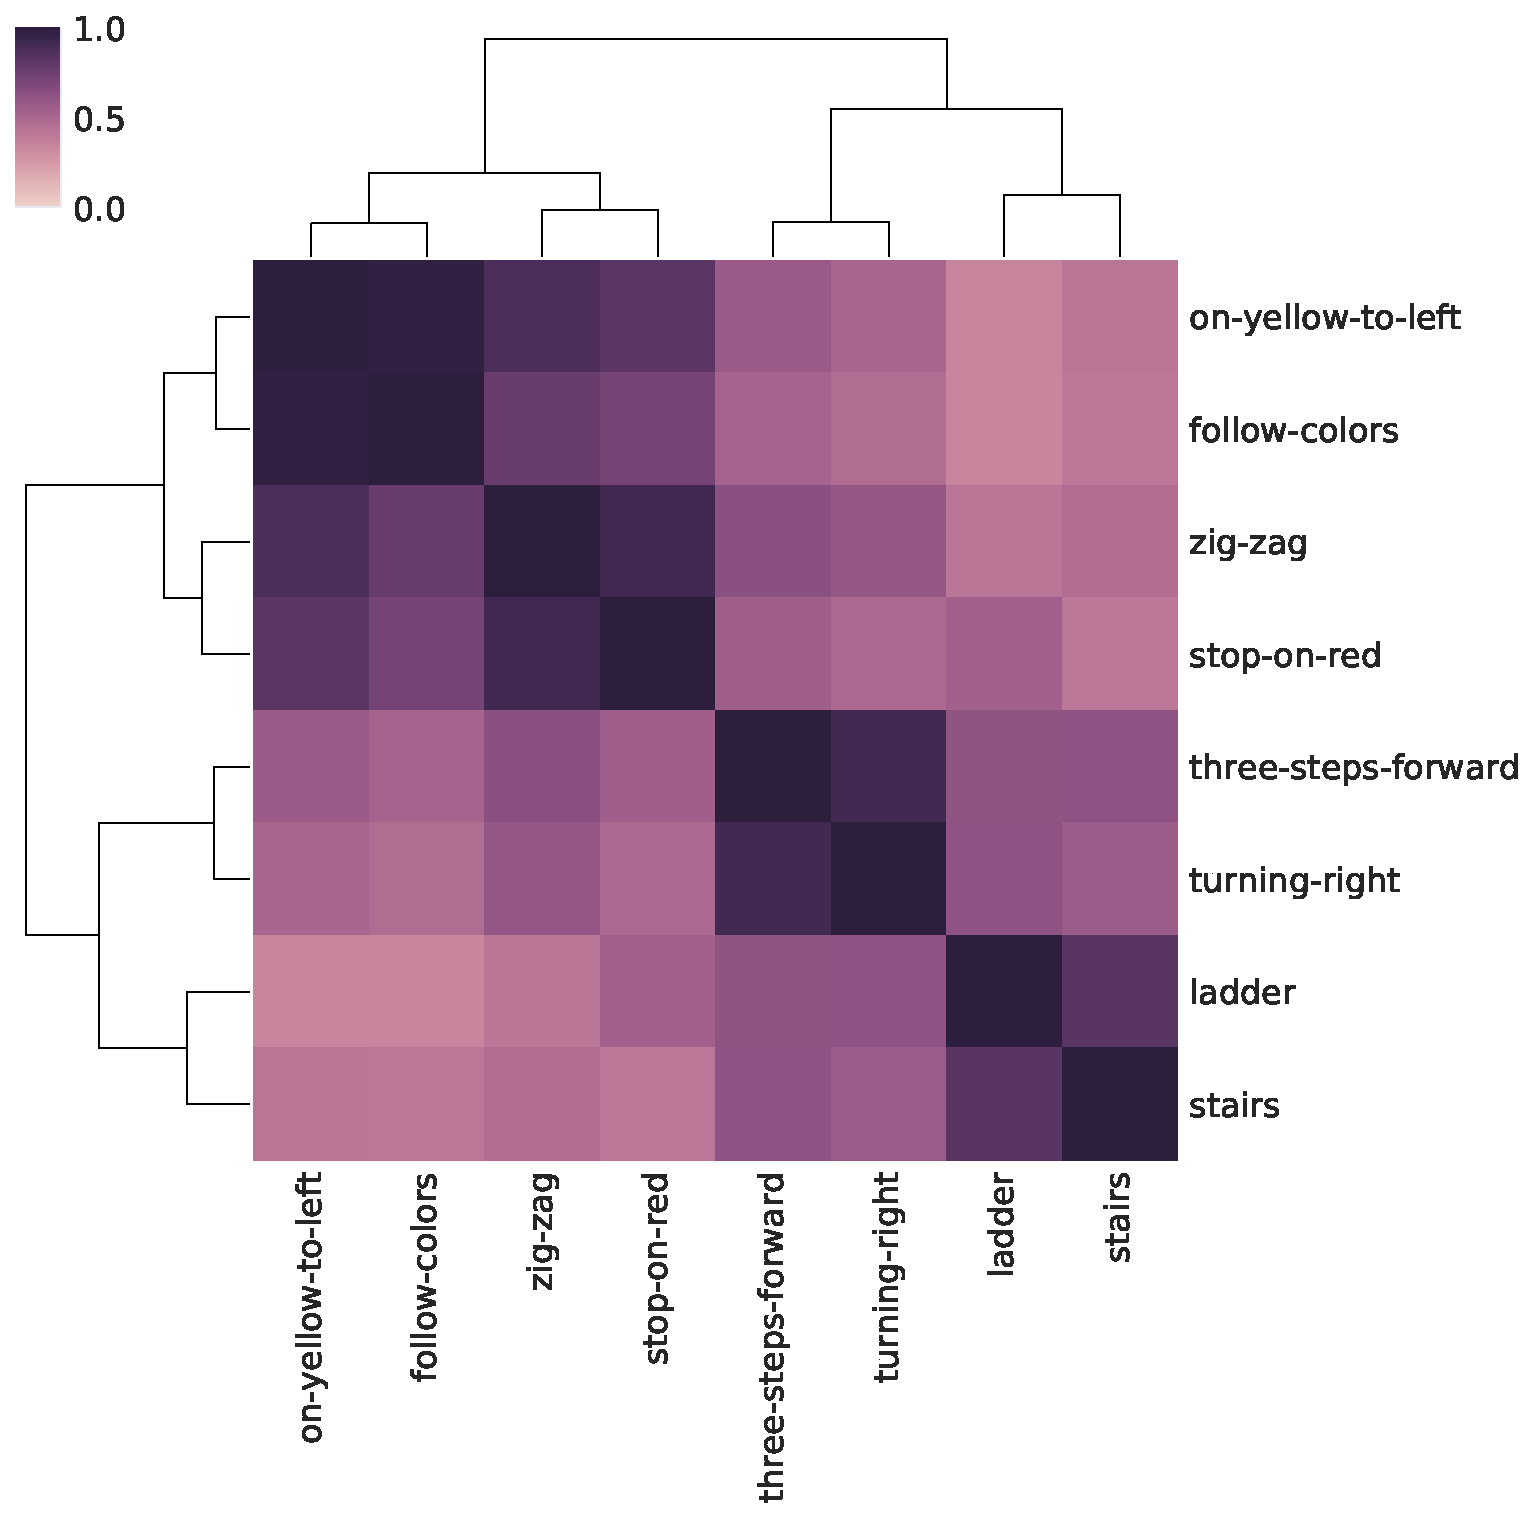
\includegraphics[width=0.48\textwidth]{img/similarities-tasks}
  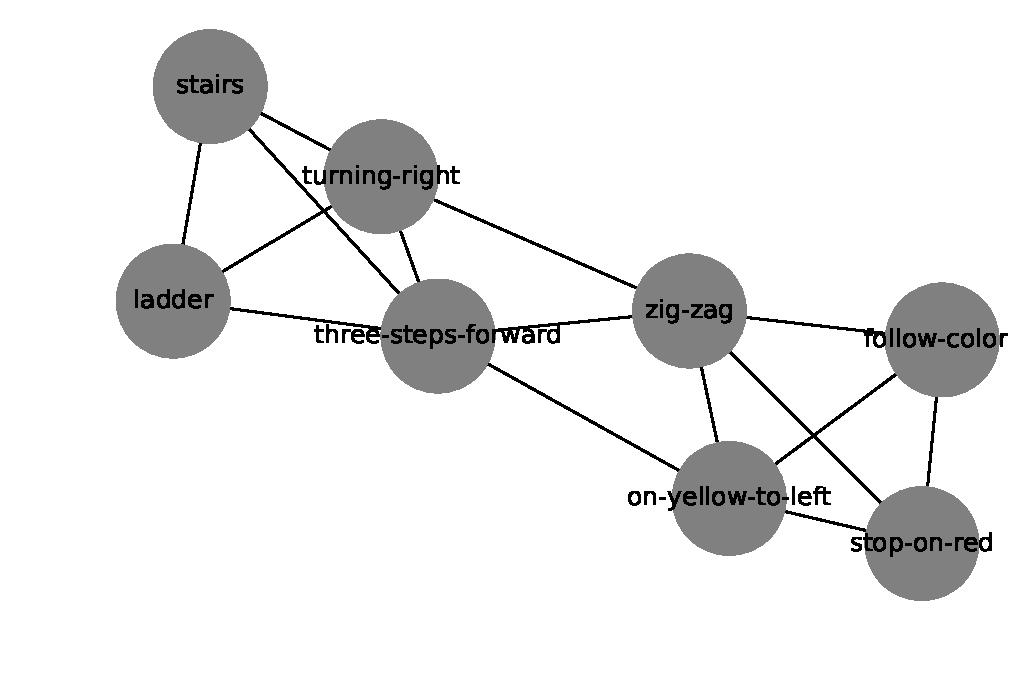
\includegraphics[width=0.48\textwidth]{img/similarities-graph}
\end{center}
\caption{%
  Left: Similarity matrix between tasks (TODO: how computed);
  right: Similarity graph with edges between tasks with high similarity.
  TODO: make it readable}
\label{fig:similarities-tasks}
\end{figure}

\subsection{Evaluation}

\begin{itemize}
\item problem: many options, which one to choose
\item again: no single best domain model depends on its intended usage
\item thus: the model should be evaluated wrt. the usage,
  which can mean we can reduce the problem of evaluation the domain model
  to the evaluation of the application -- try a bunch of different domain
  models and see their effect on the performance in the application
\item limitations:
  (1) Only works with a small number of domain models to try
  (if we want to optimize a continous parameters of the domain, then it
    is more difficult).
  (2) Requires the ability to evaluate the application, which is not
    always possible (e.g.: getting insight, open learner model) or is
    slow (e.g. requires online experiment).
\item REF to details on evaluation in the last sections of this chapter
\item TODO: illustrate: select one example of evalution and describe properly
  (some approaches to evalution are e.g. in \cite{rihak-phd})
\item TODO: example -- learning curve analysis \cite{its-domain-models}
\item example: verification of homogeneity of tasks that are assumed to be
  homogenous (interchangeable) according to current model (ie. they should
  have similar average success and solving times; statistical test testing
  that solving times comes from different distributions can be performed)
  (TODO: perform such test and illustrate, showing the two distributions
  and result of the test)
\end{itemize}



\section{Student Modeling}
\label{sec:student-modeling}

\begin{itemize}
\item Student model represents/captures
  state of the student (e.g. her skills)
  estimated from her past performance
  used to predict her future performance. (simplified)

\item Usage:
  \begin{itemize}
  \item In tutor models: (e.g.)
    recommending task of the optimal difficulty for given student,
    detecting mastery (skill of given concepts is above a threshold),
    showing hints when a student is digressing from the path towards a solution.
  \item In UI: showing feedback for the students and teachers
        (visualization of skills -- "open learner model").
  \item For online evaluation -- insight for developers (TODO: example).
  \item For offline evaluation -- insigth by researchers and programming teachers
  (TODO: example).
  \end{itemize}
\end{itemize}


\subsection{Domain vs. Student}

TODO: These are just internal notes. After incorporate clarifying comments
to relevant places, consider removing this section.

\begin{itemize}
\item The line between "domain" and "student" is fuzzy.
  It differs a lot in different papers; some even don't distinguish a separated
  domain model. (REF examples)
\item We have decided to take the following approach:
  The sole responsibility of student model is to track skills of a \emph{single}
  student. Thus, the domain model includes also population-specific parameters,
  such as initial skills, learning rate, chunk difficulties,
  precise (numeric) relationships between skills (prerequisites, mastery).
\item ?? Some of these parameters are learned within the domain model
  and then used as fixed parameters in the student model.
\item TODO: The above notes about population parameters to the domain section.
\item We could define a separate \emph{population model}, which would be useful
 if ?? we would like to model more populations and/or
 estimate the population parameters online
 (?? REF: slepe mapy - prior knowledge + difficulties estimation)
\item Note that even which chunks exist what are the relationships between them
  may depend on the population (if the population is diverse), so there is
  really no clear division on what should be a part of
  "population independent domain model" and "population model"
  (because it inherently depends on the population using the system,
  so we can decide only for the current population and provided we have collected
  enought data to analyze how large the differnces between subpopulations are
  and if it has significant impact on the application the model is used for).
\item ?? While being non-standard, we found this division to best match separation
  of concerns and thus be suitable for both explaining (as in this text)
  and impelementation (as in the developed system).
\item Domain vs Student:
  initial skills x current skills,
  concepts x skills,
  (tasks x performance),
  difficulties x skills,
  common for all students x for each student,
  offline x online.
\item Domain = state space, student = point in that space space
  (\cite{its-learner-models}).
\item example (from \cite{its-programming}):
  domain model is DAG of concepts together with a Bayesian network over this DAG
  (i.e. assignment of conditional probabilities to the edges),
  student model is (for each student) assignment from each concept to the
  knowledge (known / unknown / not-sure) -> knowlege for any concept can be
  then inferred using the Bayesian network.
\end{itemize}


\subsection{Classification of Student Models}

\begin{itemize}
\item \emph{Modeled components.}
The most explored area is skill modeling, but broader student models may also
include affect (e.g. frustration, boredom), motivation, and metacognition
(knowledge about their knowledge) (REF).
\item \emph{Underlying domain model.}
The simplest models assume either a single concept common for all tasks,
or each task as separete concept (REF: slepe-mapy). In programming,
we need to model multiple skills per task.
(REF to overlapping concepts section)
\item \emph{Granularity of skills.}
Some models track the state of the student when solving a particular task
(REF: rule-based models, constraint based models), while others
only describe the state of the student between two task sessions
(??REF: KLI framework) or even only between finished problem sets.
\item \emph{Discrete vs. continuous skills.}
Discrete = either known or not known (can have multiple levels, e.g.
unknown -> known -> fluent) (e.g. BKT); continuous (e.g. logistic models).
\cite{pelanek-learner-modeling}
\item \emph{Representation of skills.}
Instead of modeling full probability distribution of current skill, some models
only track a single point estimate,
?? or they assume a specific shape of the distribution that can be described by
a few numbers (e.g. mean and standard deviation for normal distribution).
\item \emph{Representation of performance}:
  binary correctness (solved or failed),
  discrete performance levels (e.g. poor, good, excellent),
  continuous performance (\emph{partial credit} (REF)) $p_{ij} \in [0, 1]$,
  log-time (REF: why log; possibly also REF to a relevant figure in Analysis chapter),
  or a continuous score combining time and correctness
  (see \cite[p.106]{rihak-phd} for some possible mappings).
\item ?? \emph{Predictive vs. descriptive}.
Predictive models can predict the performance of the student on a given task,
while descritive models only describe the past performance of the student.
\item \emph{Online vs. offline.}
In online models, parameters can be updated gradually after each task session
( i.e. ?? algrothm for learnining model parameters is online, REF: online algorithms).
\item \emph{Learning vs. testing.}
Models used in (??) adaptive testing (REF), assume that no learning happens
during the interaction with the system. They can be reduced to models with
learning by reestimating skills from the full student history after each task
session, but this leads to offline models.
Some models that contain learning include additional assumptions
about how the learning happens. For example, BKT (REF section)
assumes a discrete transtion from unknown state to the known state.
\item \emph{Complexity} (\cite{pelanek-learner-modeling} + TODO:page)
The more skills and relationships between them the model includes,
the more precisely it can capture the reality, but only
if there is enough data to train the model; otherwise we are in danger of
overfitting. (TODO: REF to the bias-variance tradeoff).
The number of parameters that are specific for students must be low in order to
estimate them quickly after just a few interactions of the student with the system.
(+ they are assumed to change, no older observations loose their value)
%More complex models might be also more difficult to implement, debug and interpret.
%   (?? this is a different kind of complexity; the first is size of hypothesis space)
\end{itemize}

No single best student model -- depends on the domain, intended usage, and also
on the type and amount of data we have.
In the rest of this section, we restrict our attention to the models relevant
for the domain of introductory programming and the type of the system we
are building. Specifically, we focus on models that
model only skills of concepts and predict performance on tasks,
allow for multiple skills per task,
assume learning and can be updated online.

Comprehensive overviews of student modeling:
\cite{its-learner-models, student-models-review-2012, pelanek-learner-modeling}

\subsection{Performance}

\begin{itemize}
\item Observed data from a task session:
  solved/not, solving time, number of code executions, number of edits,
  or even the individual edits (program snapshot), hints taken,
  rating or labels provided by the student (e.g. perceived difficulty).
\item TODO: mention different granularity/frequency levels for taking program
  snapshots: edits (AST changes), executions
  (REF: Educational Data Mining and Learning Analytics in Programming:
  Literature Review and Case Studies -- they differentiate more levels:
  and instead of "AST changes" they specify 2 levels ("key strokes" and
  "line-level edits"), but only the two are relevant for us (and most online,
  block-base programming environmant).
\item We first compress these \emph{observational data} into a
  single number representation of \emph{performance}.
\item The chosen representation/computation may play important role for the usage
  of the student model, e.g. in \cite{alg.mastery} they achieved better results
  in mastery learning by incorporating solving times into the performance instead
  of using just binary correctness (?? domains: math, czech).
\item Performance representation in introductory programming:
  most students solve most tasks given enough time, so correctness is out of
  question. We could still map task session data into a binary performance (1
  = good, 0 = poor), but that would not allow to distinguish between students
  for whom are the tasks just right and those for whom are too easy.
\item Three-level domain $p_{ij} \in \{0, 0.5, 1\}$ (poor, good, excellent performance)
  could already contain sufficient information for many applications
  (should be verified by future research)
  and mathces the predictions whether a given task is for given student too
  difficult, just right, or too easy.
\item Ordinal scale from definition;
  ??  It is convenient to treat it as an interval variable,
  but then it should be verified on data that the chosen compressed performance
  behaves accordingly. (TODO: explain / REF to a paper or relevant analysis in
  thesis)
\item ?? range $[0, 1]$ vs. -1, 0, 1; (disadvantage of 0-1: suggest it has interval
  scale + possible confusion with the probabilistic interpretation, which
  doesn't make much sense -- unless we assume a very specific shape of the
  probablistic distribution, we need to specify 2 numbers to get the probablity
  table)
\item Example of performance compression/extraction:
  based on solving time thresholds
  (e.g., $0.5 \times \text{median}$, $2 \times \text{median}$)
  (+ possibly REF other examples)
  (??TODO: figure -- with multiple possible representations).
\item Another option would be to model log-times (used e.g. in Tutor - REF),
  or continuous partial credit by mapping solving times to the 0-1 range
  (e.g linear fn from 0s to 2*median secs, then 0 \cite{alg.mastery}).
\item While the compression causes a loss of information,
  it also reduces noise present in the raw data.
  Most importantly, it helps to avoid a combinatoric explosion of
  considering each type of model with multiple different types of input data or
  their combination.
  Having a unified simple performance input makes the models simpler and
  easier to interpret.
\item Notation: true performance $p_{ij}$ vs. predicted performance $\hat{p}_{ij}$
\end{itemize}


\subsection{Skills}

\begin{itemize}
\item (domain vs. student: tasks -- performance, concepts -- skills)
\item ?? definition:
  $\theta_{cj} \in [0, 1]$ expresses how much student $j$ knows concept $c$
  (0 not at all, 1 mastered).
  (?? TODO: Consider using $[-1, 1]$ with 0 calibrated either to the "ready-to-learn"
  concept (flow point), or to the initial student.)
\item Possibly: not only a single point estimage, but also uncertainty,
  or even full distribution of the estimated skill.
\item Note: terms "skills" are often used interchangebly with "concepts" in
  the literature; in this thesis we strictly distinguish between "concepts"
  (independent of any student) and "skills" (associated with a student-concept
  pair).
\item Each student model thus depends ("overlays") a domain model, which
  defines a set of concepts for which to associate skills
  and describes how these skills interact among themselves and how they
  relate to each task.
\item Student models use domain as a structure,
  assigning skills (and possibly other parameters, such as uncertainty)
  to the chunks in taht structure.
\end{itemize}


\subsection{Data Structures and Algorithms}

We specify the model by its data and procedures
(as in \cite{pelanek-learner-modeling}).
We further distinguish between the historical data that are transformed into
the model data (by an online update function after each task session).

\subsubsection{Historical Data}
\begin{itemize}
\item list of task sessions
\item task session is $(t, i, j, c, p^{t}_{ij})$ with
  timestamp $t$ , task $i$, student $j$, (context $c$),
  observed performance $p^{t}_{ij}$.
\end{itemize}

\subsubsection{Model Data}
\begin{itemize}
\item underalying domain (e.g. disjunctive concepts),
\item population parameters, e.g. initial skills, learning rate,
\item skills for each student-??concept pair.
\end{itemize}

\subsubsection{Algorihtms}
\begin{itemize}
\item \emph{learning} population parameters (can be offline),
  (?? can we make population parameters part of the domain to have a single
  group of "offline-learned" parameters = domain = everything independent
  of a specific student)
\item \emph{update} of student skills based on an observed task session
  (online learning),
\item \emph{prediction} of performance for given student and task.
  (?? also prediction of skill for student-concept,
  if the data are more complex, e.g. hierarchical model?),
\item \emph{visualization} of a group of learners, e.g. learning curves
  (?? broader -- insight: also clustering of students, ...)
\item TODO: figure showing interaction between the data and algorithms.
\end{itemize}

\subsubsection{Learning population parameters}
\begin{itemize}
\item input: domain $D$, history: collected task sessions
\item output: population parameters $P$: initial skills, learning rate, ...
\item TODO: replace text by a figure
\end{itemize}

\subsubsection{Online skill update}
\begin{itemize}
\item input: domain $D$, (population parameters $P$),
  student state before the task session $\theta^{t}_{j}$,
  new task session $(t, i, j, p^{t}_{ij})$
\item output: student state (skills) after the task session $\theta^{t+1}_{j}$
\item TODO: replace text be a figure
\end{itemize}

\subsubsection{Performance prediction}
\begin{itemize}
\item input: domain $D$, (?? population parameters $P$),
  student state $\theta^{t}_{j}$, task $i$, (context)
\item output: predicted response of the student to the task,
  e.g. performance $\hat{p}^t_{ij}$
\item TODO: replace text be a figure
\end{itemize}


\subsection{Elo Models}  % TODO: Consider "Logistic models"
\label{sec:elo}

The Elo model \cite{alg.elo, irt-elo-math}
  extends the logistic model (REF, ?? IRT: \cite{irt-visual-guide})
  to capture changing knowledge.
Inspired by the rating of chess players \cite{elo-rating},
  the model interprets each attempt  to solve a task
  as a ``match'' between the student and the task.
After this match ends, skill and difficulty estimates are revised.
Depedning on whether the student solves the task better or worse than expected
  by the model, her skill is increased or decreased.
The size of the change is proportional to the prediction error -- difference
  between the predicted and the actual performance ($p_{ij} - \hat{p}_{ij}$) (``surprise'').

\begin{itemize}
\item learning rate -- not decreasing, becouse the skill is assumed to change over time
  (``nonstationary variable'')
\item note: possibility to also update task difficulties online (with
  decreasing learning rate, because the difficulties are assumed to converge)
\item The main advantage of using the Elo model is its simplicity, flexibility (TODO: elaborate),
  good prediction performance (REF) and intrinsic online nature, which allows for immediate
  updates of parameters as students are interacting with the system.
\item TODO: ?? relationship to PFA, PFAE
\item The performance predicton and udpate depends on the underlaying domain model.
  In the following sections, we discuss some of the possibilities.
\end{itemize}

\subsubsection{Single Skill Elo}

\begin{itemize}
\item underlying model: concept-free (REF)
\item TODO: formulas (?? predicting what -- continuous partial score?)
\item TODO: figure
\item TODO: relationship to EMA
\end{itemize}

TODO: formulate it within the 3-value performance (or change the performance to be between 0-1)
Elo models assume  that the probability of a student with skill $s$
?? successfully solving a task with difficulty $d$
is given by the following function:
\begin{equation}\label{eq:logistic}
P(s, d) = \frac{1}{1 + e^{-(s - d)}}
\end{equation}

\begin{figure}[h]
  \centering
  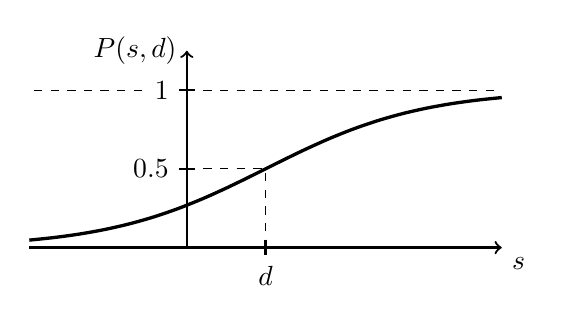
\begin{tikzpicture}[domain=-2:4, smooth, samples=20, scale=1]
  \draw [thick, ->] (-2,0) -- (4,0) node [below right] {$s$};
  \draw [thick, ->] (0,0) -- (0,2.5) node [left] {$P(s,d)$};
  \draw [thick] (-0.1,1) node [left] {$0.5$} -- (0.1,1);
  \draw [thick] (-0.1,2) node [left] {$1$} -- (0.1,2);
  \draw [thin, dashed] (0,2) -- (4,2);
  \draw [thin, dashed] (0,1) -- (1,1) -- (1, 0);
  \draw [thin, dashed] (-0.57,2) -- (-2,2);
  \draw [thick] (1,0.1) -- (1,-0.1) node [below] {$d$};
  \draw [very thick] plot (\x, {2 / (1 + exp(1 - \x))});
  \end{tikzpicture}
  \caption{One-parameter Unidimensional Logistic Model}
  \label{fig:logistic-model}
\end{figure}


\subsubsection{Multiple Skills Elo}

\begin{itemize}
\item underlying model: Disjoint Concepts / Overlapping Concepts (REF)
\item Disjoint Skills: as basic Elo but the total skill is the sum of the
global skill and concept skill (updating both the same way) (\cite{rihak-phd}, TODO: page).
\item TODO: Overlapping Skills: ?? (derivation from chosen error measure -> formulas)
\item alternative solution to the ``credit assignment problem'':
  not to update the skills directly after a failure on a single task,
  but first diagnose the issue - give the student tasks with only a subset of concepts,
  to find the problematic concept for which the skill should be decreased
  \cite{assistment-trasfer-models}
\end{itemize}

\subsubsection{Hierarchical Elo}

\begin{itemize}
\item underlying model: hierarchical model (REF)
\item REF: \cite{rihak-phd} -- assuming disjoint concepts
\item predictions: total skill = sum all ancestors skills
\item update: all ancestors sequentialy (from the top-most), elo-like update
\item TODO: formulas
\end{itemize}


\subsubsection{Network Elo}

\begin{itemize}
\item underlying model: network model (REF)
\item REF: \cite{rihak-phd}
\item each time a task is solved, update skill for all tasks according to the
similarity to the one solved (this can be propably also done on the level of
concepts, if we have a similarity network between concepts)
\item TODO: formulas
\end{itemize}



\subsection{Dynamic Bayesian Networks}

\begin{itemize}
\item underlying domain model: chunks DAG (REF)
  (?? prereqisities or also other relationships?);
\item hidden nodes = skills associated with concepts
\item observed nodes = performance on tasks
\item edges = encode dependenices (REF: BN definitional):
\item dynamic = BN with time -- each variable also depends on itslef in previous timestamp
  (before the last observation) (generalization of HMM)
\item (?? in domain): for each node have a mapping from skills/performance of children
  to skill/performance of parents (probability distribution)
\item ?? direction of edges (TODO: figure)
\item ?? approaches to model the distribution
  (discretization, assuming normal distribution for skill estimate)
\item ?? TODO: relationship between BN and Elo
  (Wang et al. 2013: Dynamic item response theory models: combining BN with logistic models)
\item ?? TODO: online update of skills after a performance?
  (to avoid repeated time-consuming skill inference)
\item TODO: formula for performance prediction ("inference in DBN")
\item example: \cite{its-programming}
\item ?? exact inference in general DBN not feasible (big network + continous distributions),
  -> ?? approximate inference (? sampling techniques),
  restrictions on the distributions and/or unerlying DAG,
  online tracking of skills (online update).
\item TODO: multiple skills: REF: Xu, Y., Mostow J.: Using logistic regression to trace multiple subskills in a dynamic Bayes Net. (LR-DBN) \cite{bn-logreg} (one-level hierarchy?)
\end{itemize}


\subsubsection{Bayesian Knowledge Tracing}
\label{sec:bkt}

\begin{itemize}
\item special case of DBN, assuming single or disjoint concepts (REF: relevant domain section)
\item (for single skill, it is even a special case of HMM)
\item for each skill, two hidden states (known/mastered) or not, observed: performance
\item assumes: learning (in contrast to basic IRT)
\item assumes: discrete knowledge state (eithter known or not known) (?! not compatible?)
\item assumes: on each opportunity to use the skill (e.g. solving a task with
  the corresponding concept), there is a constant probability of learning that skill
\item TODO: formulas for prediction and update; figure / or just REF
\item TODO: relevant extension: BKT with hiearchical model of skills
\end{itemize}


\subsubsection{AND-OR Bayesian Network}

\begin{itemize}
\item REF \cite{student-models-review-2012} (section 5.1.2)
\item REF the relevant underlaying domain mode
\item special case of DBN with assumptions on the conditional probabilities -- 2 node types:
\item OR: single mastered skill parent skill is enough to master the child skill
  (?? achieve = known = master = 1, but what about continuous skills?)
\item AND: all parent skills need to be mastered to master the child chunk
\item TODO: leaky-OR, noisy-AND; NIDA/DINA, NIDO/DINO models
\item ?? extensions to continuous skills?
\item ?? orientation of the edges (and the type of nodes in RoboMission)
\item TODO: formulas, figure / or just REF
\item TODO: consider to move to the domain model
\item TODO: discuss the relevance for our domain
\end{itemize}



\subsection{Evaluation}

\begin{itemize}
\item move there the relevant part from the Evaluation section
\item (wrt to the intended usage)
\end{itemize}




\section{Tutor Modeling}

\begin{itemize}
\item \emph{Tutor models} (aka \emph{instructional policy}, \emph{instructional
  strategy} are used to help the student with learning.
  They support the teacher by making some decisions instead of her
  (such as assigning different task to each student)
  % enabling her to concentrate on the tasks for which the people are better
  % then computers (typically inner-loop interactions, see below)
  or even substitute the teacher completely when not available
  (e.g. for home studying).
\item Includes several tasks (problems); common classification:
  within a single task session
  (\emph{inner loop}, \emph{microadaptivity}, \emph{problem solving tutors}),
  %\emph{solving process tutors}),
  or between task sessions
  (\emph{outer loop}, \emph{macroadaptivity}, \emph{problem selection tutors})
  \cite{its-learner-models}.
  Both loops can be further decomposed hierarchically
  (e.g. in outer loop: choosing a problem set to practice vs. choosing a task
  within that problem set).
  % TODO: add example for inner loop (note: not common)
  % View from \cite{its-learner-models}: inner = problem step,
  % outer = problem selection, curriculum loop = which PS).
\item Tutor tasks (control problems):
\begin{itemize}
\item \emph{Curriculum sequencing}. (?? Content sequencing)
  What topic to learn next? (What problem set to practice next?)
  Relevant for systems with a lot of diverse content with prerequisity structure.
  (e.g. in \cite{its-programming}).  % \emph{learning path}
  (Alson known as \emph{curriculum loop} \cite{its-learner-models}.)
\item \emph{Mastery learning}.
  Continue to practice the current topic or progress to another one?
  (e.g. in Umime Programovat)
% TODO: unify/clarify topic = problem set?
\item \emph{Task recommendation}.
  Which task to tackle next (possibly from a given problem set)?
 (e.g.: Tutor)
\item \emph{Adaptive scaffolding} (??).
  Should we provide the student with a help to solve the current task
  (e.g., show an instruction, a hint, a worked out example, or an explatanation)?
  (or even a suggestion to give up and try an easier task).
  (Example: cognitive tutors - REF.)
\end{itemize}
\item TODO: figure: curriculum-outer-inner loops + corresponding tutor tasks

\item Our focus is on the outer-loop.
  The inner-loop is better suited for people (instructors)
  (REF: Essa, 2016: A possible future for next generation adaptive learning
  systems.)

\item \emph{Model-based vs. model-free} (??).  % TODO: check terminology
  Often, tutor models use a domain and a student model as an input, but some
  tutors use either the full history of the student, or, on the other end of
  the spectrum, just a simple summary statistic (such as number of solved
  consecutive tasks with good performance) However, both of these cases can be
  viewed just as trivial special cases of student models) (REF).

\item \emph{Hierarchical tutor} may use different student and domain models
  for different tasks (outer loop vs. inner loop).

\item \emph{Reflexive vs. planning tutors}.
Current research and systems focus on single decision based on learned models
without a look-ahead planning.  % vs. in RL, Robotics, and CSP communities
Example to illustrate how the planning could help in task recommendation:
2 unsolved tasks left in current PS, neither of them is enough to master the topic,
the more difficult is slightly better fit to the skill; still it is better to
start with the easier one.
Example of planning for curriculum sequencing: generating a sequence of tasks
(\emph{learning path}) towards a requested topic \cite{its-programming}.

\item Output is either a single action to perform,
  (deterministic strategy/policy)
  or preferences on actions (stochastic strategy/policy).
  (Action selection for distributions: max / randomly-by-weights +
  exploration.)
  Availabele actions depend on the tutor task;
  e.g. which hint to show, which task to recommend, etc.
\item Possible representations of the tutor:
\begin{itemize}
\item \emph{Rules.}
  Mapping from conditions about states to actions, possibly with preferences.
  Each rule $R_i$ is a triple $(c_i, a_i, p_i)$
  consisting of a binary condition $c_i: S \rightarrow \{0, 1\}$,
  action $a_i \in A$, and preference $p_i \in \mathbb{R}$.
  If several rules apply, then either the one with the highest preference is used,
  or their (aggregated) preferences are used as weights for randomized selection.
  (REF)
  (Extension: ??soft/fuzzy rules: $c_i: S\rightarrow [0, 1]$)
% (?? names: rule-base tutors, production rules, expert systems) (REF).
\item \emph{Action-value function.}  % terminology borrowed from RL
  $Q: S \times A \rightarrow \mathbb{R}$.
  Function from pair of (student, action) to a score
  (prefererence -- REF to evalution section).
  For a finite amount of states, the mapping can be stored as a table,
  otherwise is approximated, e.g. through linear regression -- a weighted sum
  of some features that depend on the given student and action.
  (Rules can be transformed to action-value fn by aggregating preferences of
  all rules that trigger for current state. TODO: formula)
  (REF example)
\item \emph{Policy.}  % terminology borrowed from RL
  $\pi: S \rightarrow A$.
  Mapping from student directly to an action or distribution on actions
  (REF example)
  (Action-value fn can be streightforwardly transformed to a
  deterministic/stochastic policy.)
\item TODO ?? Other options.
\end{itemize}
\end{itemize}


\subsection{Curriculum Sequencing}

\begin{itemize}
\item Problems of curriculum sequencing:
\begin{itemize}
\item \emph{Problem set selection}: domain, student $\rightarrow$ single problem set.
\item \emph{Problem sets filtering / ranking / scoring}:
  recommend multiple PS, possibly ordered, possibly with assigned scores (how
  much they are recommended).
\item \emph{Generating learning path}: given a student and requested problem set (or a concept),
  return a (minimal) sequence of problem sets that leads to the acquiring the
  requested knowledge \cite{its-programming}.
\end{itemize}

\item Similar to task recommendation (REF section). Differences:
  much fewer problem sets than tasks,
  focus on prerequsities,
  often there even exists a reasonable total ordering of problem sets
  (consider units in a textbook).
\item Advantages of PS selection + task selection from a PS over direct task selection from all tasks in the system:
  (1) this decomposition makes the problem much simpler (both subproblems can be solved reasonably well even by simple heuristics);
  (2) focus and coherence of tasks -- students know what they are learning and does not need to adjust to very different setting every time (e.g. toolbox is not changing chaotically).

\item In a system for learning introductory programming with only a few problem sets,
  it is reasonably to assume that the student would like to "solve" (achieve mastery in)
  all problem sets. % Especially, if the UI shows which PS are solved and which not.
\item In such case, having a total ordering on all problem sets (according to their
  ``global difficulty'') and always recommending the first unsolved problem set
  is a reasonable approach.
\item If the structure is not ordinal, than we can still manually specify a
partial ordering describing which PS follow after another PS (used e.g. in UmimeX)
% ?? usually: "follow" = reversed-OR-prerequisity,
explicitly describing a recommendation fot the next PS after the current one is solved.
\item Yet another option is to specify prerequisties and recommend only PS whose
  prerequisites are satisfied.
\item The structure between PS in domains can be discovered/verified/improved using
  offline analysis of collected data, or online experiments comparing multiple options.
\end{itemize}



\subsection{Mastery Learning}
\label{sec:mastery-learning}

\begin{itemize}
\item Mastery learning means practicing of a topic (?PS) until covered concepts
  are mastered, and only then moving to the next topic.
  % "fixed outcome, varied time"
  % (vs. classical education: fixed time, varied outcome)
\item Problem: input: domain, student (skills), output: decision: mastered/not.
\item Solution: online algorithm called \emph{mastery criterion}.
\item Reduction to chosing a suitable student model \ref{sec:student-modeling}
  and a threshold $T$;
  update the student model after each interaction,
  and declare mastery when the skill
  %(probability of success or a fuzzy skill of given concept)
  on the practiced topic exceeds the threshold
  ($\theta > T$).
\item Usage of student model:
  (1) to determine if the student already achieved mastery,
  (2) to show progress to the student (progressbar).
  % TODO: screenshot of a mastery progress bar (e.g. from UmimeX)
\item Simple approaches -- using \emph{summary statistics}, i.e.
  single-concept single-difficulty descriptive student models:  % TODO: make sure the terms are defined
\begin{itemize}
\item EMA (REF EMA section in student modeling) (used in UmimeP, REF-existing-systems),
\item NCC (``N consecutive correct''), but that assumes binary performance
  (we could use something like N-with-at-least-good-performance).
  (used in KA/2018, REF-existing-systems).
\end{itemize}
\item If the problem set is coherent (tasks in PS have approximately same difficulty
  and cover the same concepts), than simple EMA works well \cite{alg.mastery}.
\item More important than chosen type of model is its input data;
  e.g. if the solving time is included in the performance (REF to performance section)
  \cite{alg.mastery}. % in the cited paper: they improved "quality" of MS by including
  % solving times over just binary correctness, ?? in both Math and Czech?
\item Disadvantage: no knowledge transfer (using the student history to improve
  mastery learning). Solution: using a sophisticated student model -- either completely,
  or just for initial setting of parameters of the simple model
  (e.g. inital score and/or learning rate and/or threshold for EMA).
\item TODO: REF some research/systems examples using sophisticated student models
  for mastery learning (hub: bibliography in \cite{alg.mastery}).
\item Parameters:
\begin{itemize}
\item threshold + parameters of chosen student models
\item Balance between overpractice and underpractice. (The righ value is application dependent.)
\item Manually: ?? using effort-score graphs \cite{alg.mastery} TODO: (elaborate)
\item Heuristically (1-step learning): e.g. require specific maximum time (e.g. 1 minute)
  to achieve mastery for genius.
\item Joint vs. 2-phase optimization
  (2-phase: for predictive models: first optimize the student model for its
  predictive accuracy, then optimize the threshold given fixed student model).
\item ?? ML wrt. to the long-short term metrics
\end{itemize}
\end{itemize}


\subsection{Task Recommendation}  % ?? "task selection"
\label{sec:task-recommendation}

\begin{itemize}
\item Problem: given domain, student, and a problem set, choose an optimal
  task from the problem set to assign to the student now.
\item Problem set: chosen by the student or curriculum sequencing tutor.

\item Types of recommenders according to outputs:
\begin{itemize}
\item \emph{task selection}: single recommended task,
\item \emph{filtering}: group of task to recommend/forbid,
\item ?? \emph{scoring}: score for each task according to how much it is
recommended,
\item ?? \emph{ranking}: ordering of tasks (all or just the most recommended),
\end{itemize}

\item \emph{Soft vs. hard recommendations}. (?? Move (partially) to UI model?)
Recommendations can be either \emph{hard}, i.e. enforced by the system
or \emph{soft}, i.e. they are presented as suggestions, but the the choice
is left on the student.
% Only a single task can be chosen as hard recommendation.
Even just showing predictions to the student (e.g. in the form of predicted
solving times or showing difficulty predictions such as
``too easy'', ``too difficult'', and ''ready to attempt'')
can be already perceived as a very mild form of recommendation.
For example, suggestions in the form of traffic-light colors
  are used in the system described in \cite{its-programming}.
Soft recommendations can be further achieved either by
  ordering tasks according to how much they are recommended,
  or only showing a subset of suitable tasks.
The system can be more strict and show only a single recommended task,
  (as in HackerRank -- REF to figure) (or 2 tasks: Tutor),
  or even enforce the recommendation by immediately progressing student to
  the next task without asking and giving them a chance to select a different task.

\item Hard and soft constraints (filters and criteria).
\item Typically hard constraints: (?? filters)
\begin{itemize}
\item Only choose tasks from given problem set.
\item Avoid already solved tasks.
\item Avoid the task which was just given up by the student.
\item (Follow the prerequisities specified in the domain.)
  (More relevant for curriculum sequencing.)
\end{itemize}
\item It is enough to simply apply all filters, unless a sequence of tasks is
  considered instead of just one. (?? In that case, the techniques from the area
  of CSP could be used -- REF.)
\item Typically soft constraints/criteria:
\begin{itemize}
\item Optimal difficulty (matching the student skills).
\item Balance diversity and coherence.
  Avoid too similar task as the previous one(s),
  especially if the student solved the task easily.
  On the other hand, do not make too "big jumps" (e.g. different toolbox or
  story in each task).
\item (?? Soft prerequisities)
\item Exploration (value of information).
\end{itemize}

\item ?? Approaches: \emph{heuristic} vs. \emph{optimized} (wrt. a metric)
  (?? learning -- online/offline).
\item Techniques (for single task recommendation):
\begin{itemize}
\item \emph{Uniform random selection}. Maximizes the exploration.
  Works well if the problem set is coherent (approximately same difficulty etc.)
  (REF usage: Umime Programovat)
\item Typical example of action-value function for task recommendation is
  a \emph{weighted sum of errors on the soft constraints}.
  Both error functions and their weights are ?usually chosen manually
  (REF usage -- MatMat?).
  In principle, the weights could be learned to optimize a desired metric, but the
  learning process is more difficult than for student models,
  because it is less clear if the decison/prediction was correct.
  (TODO: elaborate or REF to evaluation).
  (Task selection: minimizing the sum of errors / randomly-weighted)
  (Alternative combination of errors: maximum, product/sum-logs).
\item Instead of manually picking the error functions, we can directly learn
  them (e.g. via multilayer perceptron) %, or genetic algorithms, ...?
  ?? not used (or is there an example to REF?)
\item ?? Policy learning? -- e.g. a decison tree mapping student to a task
  (?? used anywhere?).
\item \emph{$\epsilon$-greedy strategy}: combination of random selection choose randomly $\epsilon$
  to balance exploration and exploitation.
\item ?? Principled approaches: MDP, weighted/fuzzy CSP
\end{itemize}
\item TODO: mention simple heuristic approach from Tutor: 2 tasks of similar difficulty as the just solved task which were not solved previously
\end{itemize}


\subsection{Adaptive Scaffolding}

\begin{itemize}
\item (inner loop)
\item ?? \emph{scaffoling} = helping student to solve a task
  (why: to make them to solve tasks slightly behind ther current knowledge to extend it).
\item ?? \emph{adaptive scaffolding} -- (vaguely) helping student during solving a task
  using automatic techniques to either generate possible hints in advance,
  or to decide when and which hint to show.

\item Possible \emph{hints} (types of scaffolding):
\begin{itemize}
\item TODO: refine terminology.
\item \emph{pre-explanations} --
  how something works, e.g. semantics of repeat-block,
  % Note: currently called "mini-instructions" in the system
\item \emph{post-explanations} --
  why something happened (REF example print-screen, e.g. that the task was not
  solved becouse the spaceship has not reached the final line),
\item \emph{worked-out examples} --
  special type of explanations, "inductive explanations",
  short programs/snippets to illustrate a concept.
\item \emph{instructions}: what to do right now
  (e.g. ``Drag and drop this block into the workspace.''),
\item \emph{interruption suggestion} --
  (special type of instruction),
  suggestion to give up and try an easier task.
\item TODO: ref examples and relevant research for all of these.
\end{itemize}

\item All of the can be to some extent used manually (i.e defining exact point in time
  and exact hints that will be shown to the student).
\item Extension points for adaptivity:
\begin{itemize}
\item \emph{hints generation} from collected history (REF),
\item \emph{just-in-time hint selection} (REF+page: \cite{student-models-review-2012})
  % note: they mention a broader category of "just-in-time feedback")
  -- algorithm that decides whether to show a hint and which one
  (using either a heuristic, such as passed time, or and inner-loop student model that capture
  possible misconceptions of the student).
\item \emph{hint personalization} -- modifying the text of hint based on the information
  about the student
  (simple example: using name of the student or their favourite characters in the text).
  (REF: there was a paper about how these simple things help for interest of the students)
\end{itemize}
\item TODO: Examples + REFs (e.g lisp-tutor)

\item Just-in-time hint selection -- how:
\begin{itemize}
\item \emph{Detecting incorrect steps.}
  Requires "ideal student model" = given the current state, what step to do
  next to solve the task.
  If diverting, show the student an instruction that forces him to get back on
  the right path leading to a solution.
  REF: lisp tutor.
\item \emph{Detecting misconceptions.}
  Requires an inner-loop student model that includes misconceptions (TODO: example)
  and showing a relevant hint to ?eliminate each misconcpetion as soon as detected.
\item \emph{Rule-based approach.}
  More generally, the tutor can include arbitrary conditions on current student state,
  mapping them to hints (and possibly preferences).
  The preferences can be then optimized e.g. using ?? buckshort heuristic (REF) (or RL, see below).
  % ?? Even new completely rules can be learned automatically, using
  % population-based heuristic search such as genetic algorthms (REF). --
  % probably not enough/useful data and you don't want to do that online...
\item \emph{Reinforcement learning.}
  Optimizing policy for an (unknown) MDP, in which
  state = student model for given task (inner loop),
  actions = possible hints (or none),
  time steps: e.g. after each edit or code execution,
  reward: e.g. +1 if solves the task (+ discount to prefer shorter paths).
  -> ?? RL techniques (enough data? used or not?)
\end{itemize}
\end{itemize}


\subsection{Evaluation}

TBA (from the evaluation section)





\section{User Interface}

TODO: consider to omit this section

TODO:
- also called "tutor-student interface"
- personalized presentation of a single task
(e.g. prefer tasks with a shooting spaceship or with ice-skating princesses,
or reference to self \cite[chapter 9]{its-domain-models})
(using information from student model)
- open learner visualization (= visualization of student model)
- personalized overview of tasks with a current recommendation (= visualization
of domain and tutor model)
- showing task recommendation (= visualization of tutor model),
  (see soft-vs-hard recommendations section)
  progress towards mastery (= tutor+student model)
  (progressbar)

\section{Metrics and Evaluation}
\label{sec:metrics-and-evaluation}


To decide if the adaptivity improves the quality of the learning system,
  suitable metrics must be chosen and evaluated.
Metrics are also used for optimizing models,
  first for parameters fitting, second for choosing hyperparameters,
  and third for selecting best model from a set of possible models.

%TODO: table/diagram showing goals hierarchy and their usage:
%1. mission -> guide for long term objectives? (not measurable)
%2. long term objectives -> AB experiments
%3. live evaluation -> spot problems ASAP
%4. offline evalution -> learn hyperparameters; holdout evaluation
%5. guide learning -> to optimize model (learn parameters, incl. only updates after new s-t interaction)

\subsection{Mission Statement}
\label{sec:mission}

There are hundreds of possible metrics that the system could measure.
What metric to choose depends on the purpose of the evaluation,
  which can range from guiding a parameters-fitting algorithm
  to interpreting results of an AB experiment.
To make sure that chosen metrics are not misleading,
  they should reflect the ultimate goal of the system,
  which is sometimes also called the \emph{mission}.

Even the mission itself should reflect some higher-level goals.
Nevertheless, goals create an infinite hierarchy
  and a starting point (called \emph{paradigm}) must be chosen,
  from which the lower-level goals are derived.
An example of such paradigm is
  ``effort to maximize the overall happiness in the population''.
% TODO: Without going into further philosophical discussions or attempts for precise definitions,
%       ... we will just adopt this paradigm for the rest of this thesis.

At first sight, a reasonable mission of a system for learning programming
  is a long-term increase in algorithmic-problem solving skill in the population.
However, other factors than the skill should be considered as well.
For example, how much students enjoyed the time in the system,
  how they are satisfied with their accomplishments,
  or if they are motivated for further learning of programming;
  all of these may play an important role for the overall happiness in the population.
In the \emph{Rules of Machine Learning}, Martin Zinkevich
  points out that there is no single best objective \cite[][Rule \#39]{google-ml-rules}.
As a solution to this ``multiple objectives dilemma'',
  the mission can be formulated as achieving a balanced increase in all
  of these important factors.
Such formulation reminds developers of the system not to overfocus on one factor
  at the cost of the others.


\subsection{Long Term Objectives}
\label{sec:long-term-objectives}

The huge disadvantage of the mission statements
  is that they are not measurable.
To make informed decisions,
  such as which of the two recommendation algorithms to prefer,
  measurable metrics are needed.
Therefore, various proxy metrics are used.
These proxy metrics should be precisely formulated and measurable,
  but at the same time they should be related as much as possible to the system mission.

To elaborate on the mission from section \ref{sec:mission},
  a long term objective could be
  ``maximizing the number of students
  who mastered elementary programming quickly while having fun''.
To make this metric usable,
  terms ``mastering elementary programming'', ``quickly'', and ``having fun''
  must be defined in a measurable way.
While ``achieving mastery in elementary programming quickly'' can be
  formulated as an objective criterion
  (e.g. ``the student solved at least 5 tasks for each concept, each in less than 5 minutes''),
  ``having fun'' requires the system to ask students about their subjective feelings.
% TODO: note that looking at the mission statement above,
% it's not clear that there must be an objective mastery criterion
% which should be achieved by all students

Furthermore, a time frame must be specified, for example last 30 days.
While short time frames allow for faster decisions and hence more improvements over time,
there are several reasons for making the time frame longer:
\begin{itemize}
  \item to collect enough data for statistical significant results,
  \item to avoid seasonality effects (such as different user behavior during weekends),
  \item to allow for more exploration, which improves long-term performance of the system.
\end{itemize}

There are many other possible long-term metrics, for example:
\begin{enumerate}
  \item Daily active users (DAU) -- students who have solved at least 1 task this day.
  \item Monthly number of active users (30DAU) -- students who have solved at least 10 tasks this month.
  \item Returning users -- students who have solved at least one task one day and have returned and solved another task another day.
  \item Converted users -- students who have finished last level in the system.
  \item Converted users -- students who have solved at least one task from each level.
  \item Number of solved tasks.
  \item Total time spent on successful attempts.
\end{enumerate}

It is not immediately clear which of these metrics is the best proxy for the system mission.
Thankfully, it was observed that at the beginning all the metrics which seem to somehow
reflect the system mission tend to improve simultaneously, no matter which one
is chosen to be directly optimized \cite[][Rule \#12]{google-ml-rules}.
To understand how their values are influenced by changes in the learning system,
it is useful to measure and report all of them from the beginning
\cite[][Rule \#2]{google-ml-rules}.

All of these suggested metrics measure a complex aggreage effect of the system
behavior during some period.
However, it is recommended to start the system optimization with a metric which is simple
and directly attributable to individual recommendations \cite[][Rule \#12]{google-ml-rules}.
The attributable metrics are presented in section \ref{sec:live-evaluation}.

% TODO: diagram of A/B testing, e.g. https://receiptful.com/blog/ab-testing-for-ecommerce
% TODO: note on AB experiments: there will be always a difference -> needs to asses statistical significance (is the difference due to changed condition or just because of random noise)
% -> t-test and similar (but mind their assumptions!) -> p-value + alpha-level -> decision
% -> add error bars to measured metrics: e.g. 95% confidence interval / standard error / standard deviation / range (+ effect size)

\subsection{Evaluation of Programming Skill}

% TODO: dichotomy between enjoyment and learning metrics - enjoyment is easier to measure (length of interaction), but learning is possibly even more important for the system mission (neither pure enjoyment nor pure learning would work -> principle of balance); measuring enjoyment -> survival analysis; measuring learning -> learning curves
% TODO: for measuring learning in AB-experiments: (pretests) and postests

The tasks environment in the learning systems usually differs significantly
  from the real-world environment,
  e.g. by using block-based programming language,
  or by other aspects mentioned in section \ref{sec:strategies-for-easier-learning}.
Ultimately, what matters is the performance of students in the real world,
  outside the simplified learning environment%
\footnote{%
  This issue is also mentioned by Weintrop and Wilensky %
  in \cite{challenges-of-blocks-based-environments}, %
  in the context of proper evaluation of block-base programming environments.}.
This aspect should be considered when choosing a proper long-term objective.
For example, trying to achieve minimum solving times on tasks in the learning system
  might be a misleading objective
  -- it would likely lead to ``overfitting'' students to the particular learning system,
  by giving them all available tasks from the simplest to the most difficult.

TODO: REF 5-week high-school experiment, block-based vs. text-based:
- \cite{comparing-blocks-text-weintrop2017}
(important feature for such comparision is to have a two learning environments,
that only differ in the text/block version of the editor, everything else being same).


\subsection{User-centered Evaluation}

In addition to quantitative (objective) metrics (such as whether the
recommended task was clicked and solved), the system can also explicitly ask
students to provide qualitative (subjective) feedback.
For example, after the student solves the task, the system can show a dialog
asking about the perceived difficulty -- whether the task was ``too
easy'', ``too difficult'' or `just right''.
Other tags about tasks can be collected as well, e.g. ``boring'', ``weird'', or ``fun''.

Collecting these tags allows to compute metrics that looks as close proxies to
the system mission, such as the total time spent in flow.
As it combines both enjoyment and learning,
flow would be a great proxy if it could be measured reliably.
% TODO: ref to a relevant research about flow

However, a known disadvantage of subjective ratings is the amount of noise
in them. They are significantly influenced by the current mood and attention of
the student.
In addition, answering these questions may bother students a little bit
and it also takes some time the students could spend on learning instead,
(but it is negligible compared to the practicing time).

TODO: quantitative vs. qualitative and online vs. field studies are othogonal,
all combinations possible: e.g. in the field study \cite{comparing-blocks-text-weintrop2017},
they measured both quantiative data (performance) and qualitative (attitude);
the same can be done in the online learning system.

TODO: note on other user-centered evaluation strategies:
questionaires, free feedback (via feedback button), user-testing (single student / class), focus groups, semi-structured interviews with sutdents.

TODO: example of a 5-week experiment in schools (field study):
\cite{comparing-blocks-text-weintrop2017}
- investigated qualities: confidence, enjoyment, perceived difficulty, interest in future opportunities to learn CS, authenticity of the environment - "is it similar to what real programmers do?", efficiency of the environment ("made me a better programmer?")

TODO: example of short user study asking for perceived quality of recommendations
(of remedial tasks) \cite{learner-models-integration-skills}

\subsection{Live Evaluation}
\label{sec:live-evaluation}

In some learning systems, a new version of a model is deployed every day
  with parameters learned from the recent data.
The behavior of the new model must be carefully monitored
  to detect problems as soon as possible,
  without waiting several weeks to evaluate an AB experiment.
For this purpose, metrics that can be linked immediately
  to the recommender actions are needed.
These metrics are called ``online attributable metrics''  % TODO: find used terminology
and this type of evaluation ``live evaluation''.

These metrics are often formulated as a question concerning a single recommendation.
To transform them into a number, either sum or average of these individual errors is computed.
% TODO: so sum or average? or some other aggregation function?

Reflecting the long-term objectives from section \ref{sec:long-term-objectives},
  there are some examples of online attributable metrics:
\begin{itemize}
  \item Was the recommended task chosen by the student?
  \item \ldots and did the student solved the task?
  \item \ldots in a reasonable time (e.g. 1-15 minutes)?
  \item \ldots and did not the student marked it as ``too easy'' or ``too difficult''?
\end{itemize}

% TODO: relationship to metrics defined in section \ref{sec:metrics-for-recommendation}

% TODO: note on online models (and relation to RL), these needs continuous online evaluation

% TODO: taking delta wrt. previous model

TODO: note on multi-armed bandits (special case of RL with a single state) as
an alternative to AB experiments that deals with the exploration-exploitation
tradeoff; (description in the context of ITS: \cite[p.129]{its-domain-models}).

\subsection{Offline Evaluation}

Offline experiments use historical collected data
  to avoid the cost of live evaluation.
The advantages of offline experiments compared to online evaluation include
  the possibility to run as many experiments as needed,
  obtaining the results quickly,
  reusing the same data to evaluating different models,
  and avoiding potential negative impact on students if the evaluated model is poor.

Of course, offline evaluation is limited,
  because there are not all the historical data needed
  for proper evaluation.
For example, when evaluating a new recommendation algorithm,
  the data about a student responding to a particular recommendation
  are often not available.
Another disadvantage of offline evaluation compared to live evaluation
  is that the data used for evaluation does not come from the completely
  same distribution of events as will occur in the live system,
  which limits generalization guarantees of such evaluation.
% TODO: note: further decrease of relevance to the system mission - but worth

Offline evaluation is typically used as a check before pushing
  the model online to avoid problems as soon as possible.
It can also be used for model selection,
  including hyperparameters search.
Finally, offline learning algorithms typically also use
  a metric to guide them
  (these are discussed in section \ref{sec:metrics-to-guide-learning}).


TODO: comparing to other (e.g. currently used) model (e.g. correlation between predictions, delta between recommendations):
1. for a prototype (idea) of new model: if the correlations are high, there is probably no significant gain in exploring this model (compared to using the current one);
2. for same model with retrained parameters for newly collected data - if the delta is too big, we should be suspicious and investigate.

TODO: evaluating parameters stability (see thran-thesis) - as above just with the same model (comparing the same model trained on different samples from the collected data)

\subsection{Cross Validation}

TODO: consider removing this section and only point to a relevant description
of CV in the context of student models evaluation, e.g. in \cite{pelanek-learner-modeling}
(our main scenario/methodology: "online evaluation with generalization to new learners")

Trained models must be evaluated on data unseen during training.
Straightforward approach is to split collected data into two parts,
  first used for training (\emph{training set})
  and second for evaluation (\emph{test set}).
To use data more efficiently, the train-test split can be repeated
  $k$ times, taking different $1/k$ portion of the data for testing every time,
  and computing averaged performance.
The described method is called \emph{cross validation}.

While random train-test split over all training examples works often
  best in many machine learning domains,
  one must be careful when dealing with data from learning systems.
A completely random split would lead to predicting past performance
  of student from the model trained on their future performance,
  which could result in over-optimistic results.
The recommended splitting technique is ``user-stratified'',
  in which we randomly split students,
  and create training set from all events of one group of students,
  and first $n$ events of all students in the second group.
The test set then contains $(n+1)$-th events from the students
  in the second group.
The evaluation can be repeated for all possible $n$'s and averaged.
This is simple and fast for online models
  (that can be trained iteratively by one training event),
  but it is more involved and often too slow for offline models.
To make the evaluation reasonably fast,
  some simplifications can be used,
  such as predicting not only one, but multiple events
  for each student in the second group during a single split.

% TODO: make it clear that even for online models, we are still discussing offline evaluation
% TODO: discuss compromises for evaluation of offline models (or point out to a relevant paper)

If the model contains hyperparameters to select,
  it is important to use yet another non-overlapping portion
  of data for hyperparameters search,
  which used neither for training, nor for final evaluation.
This third portion of data is sometimes called \emph{validation set}
  (though the terminology for this is not unified).
Cross validation can be generalized to account for this 3-parts split
  and the resulting method is called \emph{nested cross validation}.

% TODO: figures to illustrate all the described methods and splits

NOTE: \cite{student-models-review-2012} also discusses the "correct level on
which to perform the cross-validation": never on the level of individual
"actions" (task sessions), but rather on the student level (to see how the
system will behave for the new students in the system, for which it wasn't
pretrained offline), sometimes it make sense to use the "chunk level"
(to see how it generalizes to new chunks), "school levels" (new populations of
students)
(in sklearn this is called "Group k-fold cross-validation")

\subsection{Student Model Evaluation}
\label{sec:student-model-evaluation}

A student model (described in \ref{sec:student-modeling})
  is an important component for adaptive learning techniques
  such as recommendation algorithms.
Therefore it is reasonable to believe that optimizing the quality
  of used student models should result in better recommendations
  and transitively in improving the long-term objectives.
Although better predictions usually help,
  the relationship between their quality and the long term objectives
  is not always straightforward.
If the online experiments show that the more accurate predictions would actually
  lead to decrease of the long-term objectives,
  then these improvements in the predictive power should not by applied.

The next two sections present metrics for two most common
  types of student models according to their output:
  predicted solving times and predicted success.
% TODO (consider): generalize: any real values (e.g. times)
%                  vs probabilities (success, too-difficult)


TODO: Student models are used for different purposes
(e.g. inner loop, outer loop (task recommendation) human-in-the-loop (insight),
open learner visualization, )
evalution should reflect the intended purpose
(see \cite{pelanek-learner-modeling}).

NOTE: overview of metrics for student models comparison, e.g. in \cite{pelanek-evaluation-student-models}

TODO: reliability and resolution of predictions (also in \cite{pelanek-evaluation-student-models})

TODO: reliability/stability of parameters

TODO: "plausibility of parameters" \cite{learner-models-integration-skills}


\subsection{Metrics for Time Predictions}
\label{sec:metrics-for-time-predictions}

% TBA: note on data we need (and easily collect in this case)
To evaluate the quality of solving times predictions,
  vector of predicted times $\hat{t}$ is compared to
  the vector of true observed times $t$.
Usually, individual errors between tuples $(t_i, \hat{t}_i)$ are computed
  and then averaged.
While it is possible to take an absolute value of the
  difference $(t_i - \hat{t}_i)$,
  which results in Mean Absolute Error (MAE),
it is more common to taking square of the difference
  to penalize more one large error than multiple small ones.
In this case, it is common to take a square root of the final
  average, to bring the units back to the original ones
  for better interpretation.
This metric is called Root Mean Squared Error (RMSE).

$$
RMSE(t, \hat{t}) = \sqrt{\frac{1}{n} \sum_{i=1}^n (t_i - \hat{t}_i)^2}
$$

Note that the solving times should be first log-transformed;
  otherwise a single outlier could make the error extremely high.
% TODO: provide more details/ref to an earlier section about taking logs
% TODO: also note that these type of metrics will be always susceptible to
% outliers anyway

% TODO: Statistic notes why the RMSE makes sense:
%       - explain that given some assumption
%       -> results in best linear estimator
%       - and even MLE (assumption of normally distributed noise),
%                       -> it's equivalent to RMSE - see Bishop, 2006)

%TODO: The metrics presented in this section
%  can be also used for evaluation of other real-valued predicted variables,
%  such as flow (if formalized to take real values.)


\subsection{Metrics for Success Predictions}
\label{sec:metrics-for-success-predictions}

Some student models predict a probability that
  a given student would solve a given task.
% TODO: statistics terminology - alternative distribution
In this case, each the true labels are not any real number,
  but just zeros and ones.
This difference is important for the choice of a suitable metric.
Good overview of possible metrics is presented in \cite{pelanek-evaluation-student-models},
  which also shows a simple example demonstrating why MAE should not be used
  as an error measure for binary predictions.
In addition to RMSE, Log-Likelihood (LL) is sometimes used:
$$
LL(s, \hat{s}) = \sum_{i=1}^n s_i\log(\hat{s}_i) + (1-s_i)\log(1-\hat{s}_i)
$$
% TODO: include derivation of LL from MLE principle (product -> log -> sum)
Note that LL differs from RMSE in several aspects.
First, as opposed RMSE, the higher LL the better,
second, it is negative,
and third, it is not averaged, so it decreases with the size of data set.

The RMSE and LL are based on a probabilistic view of errors.
There is another set of metrics based on the qualitative understanding of errors,
  which compares the observed success with binarized predictions,
  instead of real-valued probabilities.
For example, \emph{accuracy} is a ratio between correct predictions to all predictions.
However, these metrics do not distinguish between small and large errors of the predictions,
  which makes them less appropriate for student modelling.

% TODO: details, possibly table of common metrics from the confusion matrix
% (precision, recall, sensitivity, specificity, ...)
% TODO: mention: allows for setting different risks (weights) on different types of errors
% TODO: diagram: comparison of these individual errors, see pelanek-evaluation-student-models, p.6

These error metrics depends on a particular threshold chosen
  for binarization of predicted probabilities.
There are metrics avoiding this problem by using only ranking of predictions.
The most common one is AUC, ``Area Under Curve'',
  which is the probability that if one failure and one success are selected by random,
  the predictor would assign a higher probability to the success event than to the failure.

There are a few limitations of AUC.
First, it considers all thresholds, but only a range of them is usually relevant.
Second, by only considering the ordering of predictions,
  if all predictions are multiplied by a constant, AUC remains unchanged.
Third, if the predicted classes are strongly imbalanced,
  high AUC can be achieved by simple classifiers
  even if they perform poorly on the minority class.
Generally, AUC is a reasonable choice for intrinsically classification problems,
  but not necessarily for student modeling \cite{pelanek-evaluation-student-models}.

% TODO: precise definition of AUC using ROC curve
% TODO: check if the intuitive explanation of AUC is correct
% TODO: how to deal with the limitations: global objectives (ranges of thresholds), AUC-PR for unbalanced problems

\subsection{Offline Evaluation of Recommendations}

% TODO: consider moving before metrics for predictions?

Offline evaluation of recommendation algorithms is considerably more difficult
  than evaluation of student models.
The reason is missing data --
  if the evaluated algorithm recommends a task $t$ to student $s$
  in a specific point of his learning process (e.g. after first 2 solved tasks)
  but the student $s$ attempted different task at that point,
  there is no easy way to tell if the recommendation is good or not.

The extremeness of data sparsity makes offline evaluation so challenging,
that most learning systems completely skip this type of evaluation,
apply offline evaluation only to student models
(section \ref{sec:student-model-evaluation})
and check quality of recommendation algorithms on live traffic
(section \ref{sec:live-evaluation}).

Nevertheless, realizing that the offline evaluation serves just as another proxy metric,
  it may be still useful to perform at least some limited offline evaluation
  before putting the recommender to the wild of real world.
There are some possible approaches:
\begin{itemize}
  \item For each recommendation event in the collected data,
      look if the recommended event is among one of top $N$ (e.g. 10) tasks
      recommended by the evaluated recommender
      and compare it with the observation whether this particular recommendation
      was good (e.g. whether the student attempted and solved this recommended task).
      (These comparisons can be turned into several different metrics,
       which are described in section \ref{sec:metrics-for-recommendation}).
      % TODO: point to a section with confusion matrix, precision, recall etc.
  \item Instead of looking at the past recommendations,
      events when students themselves selected a task from a list of all tasks can be used.
      (It is also possible to combine both recommendation and self-selection events
       as a single dataset.)
  \item Prepare a small manually labeled dataset describing appropriate and
    inappropriate recommendations for given combination of features, possibly
    by extending collected data on recommendation.
  \item Measure agreement in recommendations between a new recommender and one which is already used and was evaluated on live traffic (recommended by \cite[][Rule \#24]{google-ml-rules}).
\end{itemize}

% TODO: note on data bias in most of these approaches

\subsection{Evaluation of Mastery Learning}

TODO: Effert vs. Score plot/metrics \cite{learner-models-integration-skills}

\subsection{Metrics for Recommendations}
\label{sec:metrics-for-recommendation}

There are multiple metrics that can be used for both online and offline
evaluation of recommendations.
These metrics can be divided into several categories
according to what data they need.

For a series of student-task interactions paired with a recommendation list of
fixed length $N$, a \emph{confusion matrix} can be constructed by comparing
whether the interaction was beneficial for the student or not,
and whether the task was within top $N$ recommended tasks.
Having the confusion matrix allows to compute various metrics such as
accuracy, precision, or recall. % TODO: or sensitivity/specificity/... + define

Depending on the user interface, fixed $N$ might or might not make sense.
If not, it is possible to use more sophisticated metrics without a fixed $N$,
such as AUC (described in section \ref{sec:metrics-for-success-predictions}),
or MAP (Mean Average Precision).
% TODO: MAP = AUC-PR?
% TODO: or DCG?

In some cases, for example when comparing two recommendation algorithms,
complete lists of ordered tasks are available.
In this case, other \emph{ranking metrics},
  such as Spearman's rank correlation coefficient,
  or Kendall's rank correlation coefficient,
  can be also used.
% TODO:  Discounted cumulative gain, average precision, lift index, ...

%# Beyond simple accuracy
All these metrics focus on accuracy of the recommendations,
but there are other properties of recommendation algorithms,
which may influence its usefulness for students,
such as robustness or diversity.
% TODO: note: but they are more difficult to express/measure,
% so they are used much less in practice

For example, if the system shows several recommended tasks,
but these are all nearly identical, there is no added value
for the student from the possibility to choose from them.
Similarly, if the student has just solved a task
without any problem, the next recommended tasks should
differ considerably not to be boring for the student.
To measure similarity between tasks, their content features
constructed from their statement and solution are compared
using some distance metric.
% TODO: ref to our current item-similarity research


\subsection{Metrics to Guide Learning}
\label{sec:metrics-to-guide-learning}

Learning algorithms often incorporate a metric they attempt to optimize.
In this context, the metric is often called \emph{loss function}.
For example,
  Ordinary Least Squares (used for linear regression models) minimizes RMSE.
Some learning algorithms, such as gradient descent,
  allow to minimize arbitrary metric
  for which it is easy to compute partial derivatives with respect to model parameters.
Loss functions can be viewed as just further proxies for long-term objectives.
Therefore, in the case of choice, it is beneficial to choose a loss function
  that matches the long-term objectives more closely.

As a common example, some loss functions allow to specify weights for each training example.
If it is derived from the long-term goals that predicting one class correctly
  is more important than predicting the other class correctly
  (e.g. if it is more important to predict correctly failure than success),
  larger weights should be assigned to the examples with the more important class.

Note that these metrics are not limited to the offline environment. Specifically, if the
model only process each student-task interaction once (\emph{online models}), than the
model parameters can be updated based on the value of the error metric
(or its gradient in the case of gradient descent) in the live environment.

\subsection{Simulation Experiments}

Online experiments relies on live data,
while offline experiments use historical data.
Simulated experiments provide a third alternative,
  which does not require any collected data at all.

Not needing collected data makes simulations widely and easily applicable.
On the other hand, researchers must be careful when interpreting
  the results of a simulation, as the simulation results are nothing more than
  just consequences of used assumptions.
Nevertheless, simulation are perfect for models debugging,
  for example to find fatal errors in the implementation.
Furthermore, \emph{sensitivity analysis} is a technique for finding
  which parameters of the model are important and should be learned,
  and which can be safely set manually without frequent retraining.

In practice, simulations can also take advantage of collected data
  if they are available -- to estimate some of the model parameters
  or to evaluate how much the model predictions agree with
  what was observed in the reality.


TODO:
- view on the simulation experiments as the 3rd way between deduction (mathematical models) and induction (statistics, machine learning)
- REF examples (e.g. in thran-thesis)
- they can also provide best-case performance, suggest how much data (at least) is needed to achieve stability/good performance



\subsection{Data Collection}

TODO: overview of issues e.g. in \cite{pelanek-learner-modeling}

TODO: attrition bias (type of selection bias, can be caused by self-selection)

TODO: Feedback Loops
% TODO: describe the bias: recommenders -> influence collected data ->
% evaluation on the data influenced by them; (big issue in recommendation
% systems in general)
% TODO: give an example (including the resulting problem)
% TODO: REF: Google Rules of ML 36


\subsection{Iterative Improvement}
\label{sec:iterative-improvement}

Importance:
- importance of iterative improvement in general (rule of the loop -- REF: book of lenses)
- specifically in ML -- REF Google Rules of ML 16: "Plan to launch and iterate"
- specifically in ITS: REF
- specifically for domain models: recommendation from \cite[p.124]{its-domain-models}:
"Treat each domain model as a hypothesis rather than a perfect final definition. (...)
Facilitate iterative improvement of domain models."

TODO: How:
- important components mentioned in the above sections:
  monitoring (metrics), performing AB-experiments, live evaluation, offline
  analysis
- offline analyses -- the term ``human in the loop''
\cite{stupid-tutoring-systems-intelligent-humans}

TODO: examples:
- start with the initial ("expert-provided") domain model -> collect data ->
analyse -> refine -> iterate (\cite[chapter 10]{its-domain-models})

